%!TEX root = ../main.tex

\section{Hardware Description}
Many parts are involved in making the go-kart drive.
This section will give a short description of each part in order to make an overview of the system.

\subsection{Go-Kart Frame}
The Go-Kart itself consists of a pre assembled aluminium frame with wheels, steering column, break pedal and seat all pre-attached to the frame. 
A plate is attached behind the seat to fit all of the power electronics and drive systems that are designed throughout this project.
To the right of the driver a mount is positioned for the motor.
The mount is protected by a metal cover. 
In order to transfer power to the rear wheels, a gearing is placed between the motor and the rear axle.
A conventional disc brake comes pre-installed on the kart with the break pedal connected using hydraulics.
The torque pedal is also installed, but with no mechanical effect on the system.

\begin{figure}[!h]
	\centering
	\includegraphics[width=.35\textwidth]{graphics/Gokart_Frame}	
	\caption{The frame of the Go-kart used in the project.}
	\label{fig:Kart_picture1}
\end{figure}

\subsection{Battery Supply}
The batteries provided for this project are of the type SB12V20P-FC \cite{battery_datasheet}.
Four of these batteries are put in series, yielding a combined nominal voltage of 52.8V and a discharge current of 560A. 
The discharge current can go as high as 1200\si{\ampere} for one second.
The batteries will be providing all the required power for the go-kart, including the motor and all control and drive circuits.

\subsection{PMAC Motor}
The PMAC motor provided is a three phase motor capable of producing 6hp continuously and a peak power of 19hp for a minute, at a maximum rotational speed of 5000rpm. 
It has an efficiency of 90\% and a stall torque of 38Nm. Its typical uses are, among other things, marine, robotics and go-karts.

\subsection{Torque Pedal}
The foot pedal or "speeder" will be used to control the torque produced by the motor and will henceforth be referred to as a torque pedal. 
It consists of a levered variable resistor with the electrical diagram seen in figure \ref{fig:Torque_pedal_diagram}.

The torque pedal will be used to control the torque by altering the resistance, resulting in a change in voltage on the return wire. 
By measurement, it is found to have a variable resistance of 0\si{\kilo\ohm} to 7.5\si{\kilo\ohm}.
By nature a variable resistor is noisy therefore filtering the signal will be necessary.

\begin{figure}[!h]
	\centering
	\begin{subfigure}[t]{.35\linewidth}
			\includegraphics[width=\textwidth]{graphics/torque_pedal_diagram}
			\caption{Diagram of the torque pedal.}
			\label{fig:Torque_pedal_diagram}
	\end{subfigure}
	\hspace{2cm}
	\begin{subfigure}[t]{.35\linewidth}
		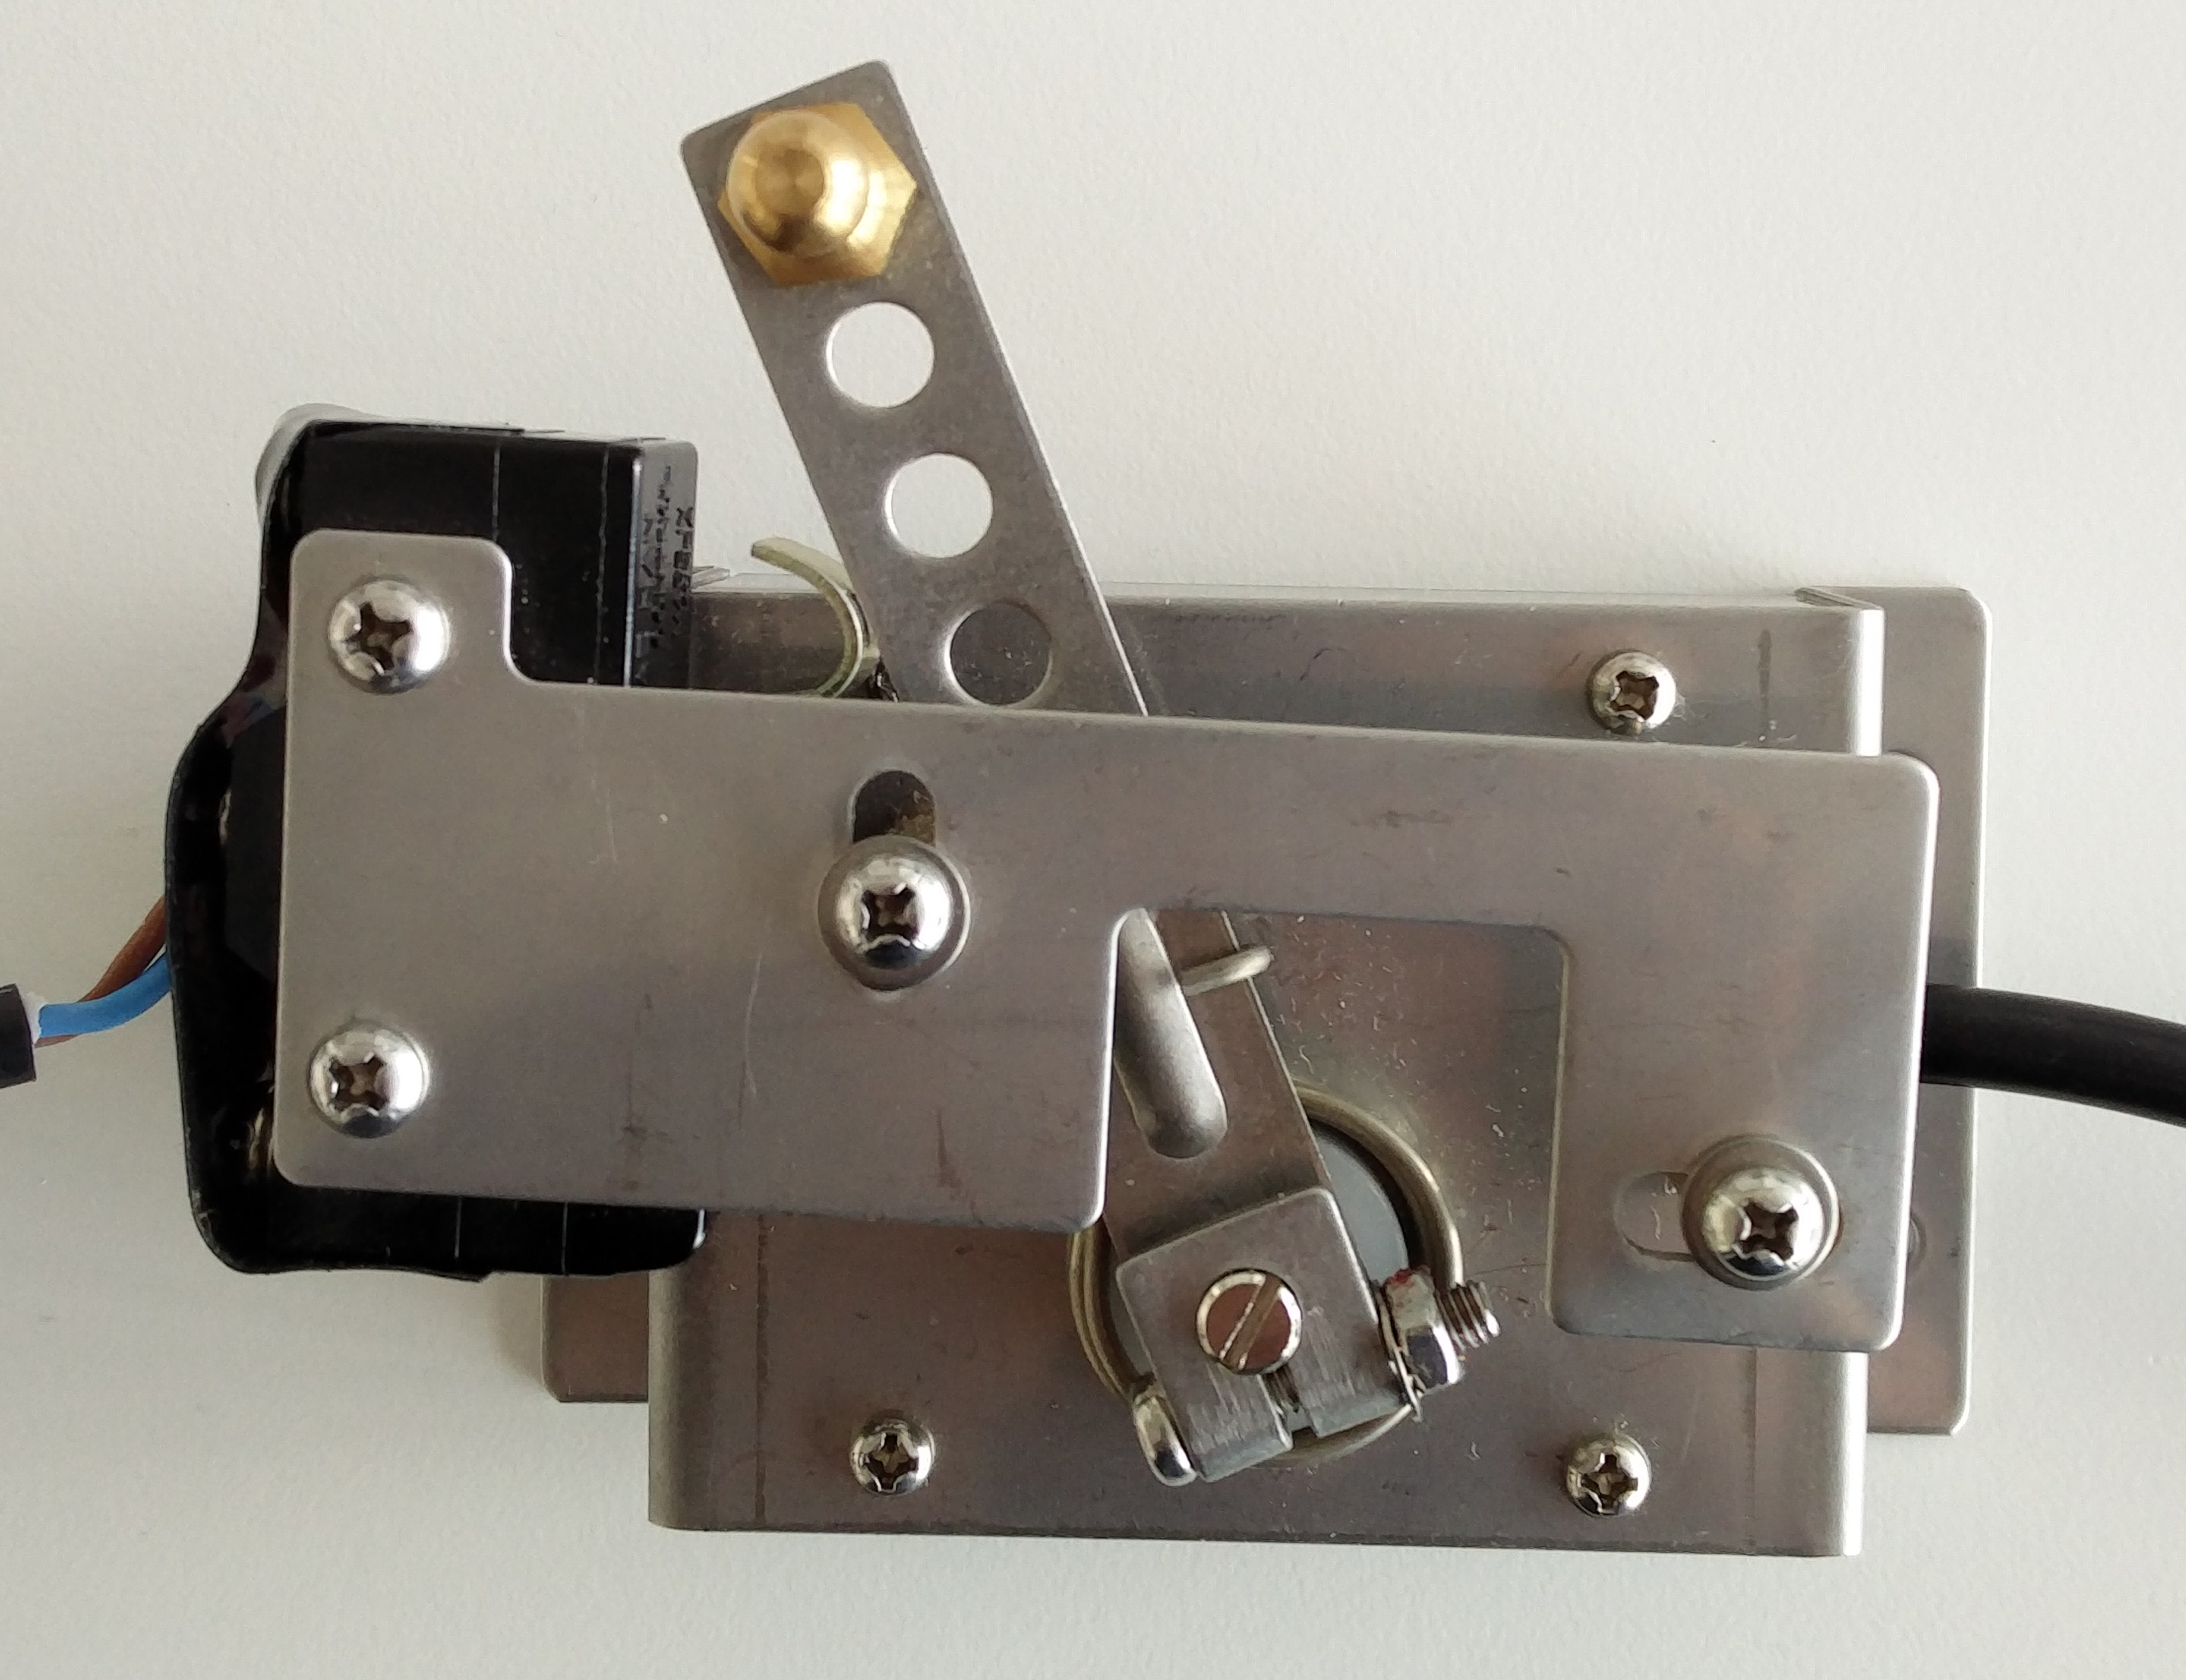
\includegraphics[width=\textwidth]{graphics/torque_pedal_picture}
		\caption{Picture of the actual torque pedal.}
		\label{fig:Torque_pedal_picture}
	\end{subfigure}
	\caption{Diagram and picture of the torque pedal.}
	\label{fig:Torque_pedal_diagram_and_picture}
\end{figure}

\subsection{Switches and Wiring}
The wiring of the kart frame is not pre-assembled, but has been provided by the supervisors of the project.
A diagram of the wiring can be seen on figure \ref{fig:Kart_wiring_diagram}.\newline

The diagram shows the Sevcon Gen4 controller as the centerpiece surrounded by the other active parts. 
The motor to the right. 
The torque pedal, battery, undervoltage protection and multiple switches to the left. 
The switches include a key switch to turn the system on, an emergency switch, and a drive enable switch with three positions to change between driving forwards, reversing or disabling drive at the neutral position.
\todo[inline]{Change orientation of figure}
\begin{figure}[!h]
	\centering
	\includegraphics[width=.95\linewidth]{graphics/Electrical_wiring_diagram_ver3}
	\caption{Go-Kart wiring diagram.}
	\label{fig:Kart_wiring_diagram}
\end{figure}

\clearpage